\documentclass[a4paper]{article}

\usepackage[english]{babel}
\usepackage[utf8]{inputenc}
\usepackage{amsmath}
\usepackage{graphicx}
\usepackage[colorinlistoftodos]{todonotes}
\usepackage{hyperref}
\usepackage{listings}
\usepackage[numbers]{natbib}

\usepackage{booktabs} % To thicken table lines



\title{Creating Customer Segments}

\author{Uirá Caiado}

\date{\today}

\begin{document}

\maketitle

\begin{abstract}
As pointed out by \cite{Udacity}, today many companies collect vast amounts of data on their clientele and have a strong desire to understand the meaningful relationships hidden in their customer base. In this project, I will apply unsupervised learning techniques on product spending data collected for consumers of a wholesale distributor in Lisbon, Portugal. My goal is to define how best segment their customers into distinct categories. Afterwards, the segmentation found will be compared with an additional labeling. Lastly, I will suggest ways that the segmentation could assist the wholesale distributor with future service changes.
\end{abstract}

%%%%%%%%%%%%%%%%%%%%%%%%%%%%%%%%%%%%%%%%%%%%%%%%%%%%%%%%%%%%%%%%%%%%%%%%%%%%%%%%%%%%%%%%
%% INTRODUCTION
%%%%%%%%%%%%%%%%%%%%%%%%%%%%%%%%%%%%%%%%%%%%%%%%%%%%%%%%%%%%%%%%%%%%%%%%%%%%%%%%%%%%%%%%

\section{Introduction}
\label{sec:introduction}
In this section, I will give some background about the problem addressed and the goal of the project.

\subsection{Some Background}
As suggested by this article\footnote{Source: \url{http://goo.gl/aEqNpD}}, the current abundance of digital data from many sources — the web, sensors, smartphones and corporate databases — can be mined for discoveries and insights and might lead to smarter, data-driven decision-making in every field.

In this project, I will analyze a dataset containing data on various customers' annual spending amounts of diverse product categories looking for internal structure. One goal of this project is to best describe the variation in the different types of customers that a wholesale distributor interacts with. Doing so would equip the distributor with insight into how to best structure their delivery service to meet the needs of each customer.

Given that there is no previous labeling of each instance in the dataset, I will use unsupervised learning to look for such structure. As explained by \cite{Mitchell}, in this case, there is a set of $N$ observations $(x_1,x_2, ..., x_N )$ of a random vector $X$ that has a joint density $Pr(X)$. The goal is to directly infer the properties of this probability density without the help of a supervisor or teacher providing correct answers or degree-of-error for each observation.

\subsection{Getting Started}
The dataset for this project can be found on the UCI Machine Learning Repository\footnote{Source: \url{https://archive.ics.uci.edu/ml/datasets/Wholesale+customers}}. For the purposes of this project, the features \textit{'Channel'} and \textit{'Region'} will be excluded in the analysis — with focus instead on the six product categories recorded for customers. So, let's start loading the dataset:

% code snipet
\begin{lstlisting}
Wholesale customers dataset has 440 samples with 6 features
each.
\end{lstlisting}

%%%%%%%%%%%%%%%%%%%%%%%%%%%%%%%%%%%%%%%%%%%%%%%%%%%%%%%%%%%%%%%%%%%%%%%%%%%%%%%%%%%%%%%%
%% DATA EXPLORATION
%%%%%%%%%%%%%%%%%%%%%%%%%%%%%%%%%%%%%%%%%%%%%%%%%%%%%%%%%%%%%%%%%%%%%%%%%%%%%%%%%%%%%%%%


\section{Data Exploration}
\label{sec:data_exploration}
In this section, I will begin exploring the data to understand how each feature is related to each others. The six labels explored are continuous and are related to the annual spending on diverse product categories. They are all expressed in in monetary units. The features are:
\begin{itemize}
\item FRESH: fresh products 
\item MILK: milk products
\item GROCERY: grocery products 
\item FROZEN: frozen products
\item DETERGENTS\_PAPER: detergents and paper products
\item DELICATESSEN: delicatessen products
\end{itemize}

In the Table \ref{tab:basicfacts} below can be observed a statistical description of the dataset:

\begin{table}[ht!]
\centering
\begin{tabular}{l|rrrrrr}
{} &      Fresh &      Milk &   Grocery &    Frozen & Detergents\_Paper & Delicatessen \\\hline
count &     440.00 &    440.00 &    440.00 &    440.00 &           440.00 &       440.00 \\
mean  &   12000.30 &   5796.27 &   7951.28 &   3071.93 &          2881.49 &      1524.87 \\
std   &   12647.33 &   7380.38 &   9503.16 &   4854.67 &          4767.85 &      2820.11 \\
min   &       3.00 &     55.00 &      3.00 &     25.00 &             3.00 &         3.00 \\
25\%   &    3127.75 &   1533.00 &   2153.00 &    742.25 &           256.75 &       408.25 \\
50\%   &    8504.00 &   3627.00 &   4755.50 &   1526.00 &           816.50 &       965.50 \\
75\%   &   16933.75 &   7190.25 &  10655.75 &   3554.25 &          3922.00 &      1820.25 \\
max   &  112151.00 &  73498.00 &  92780.00 &  60869.00 &         40827.00 &     47943.00 \\

\end{tabular}
\caption{\label{tab:basicfacts}Statistic About the Dataset.}
\end{table}

\subsection{Bla}
bla bla.

\begin{figure}[ht]
\centering
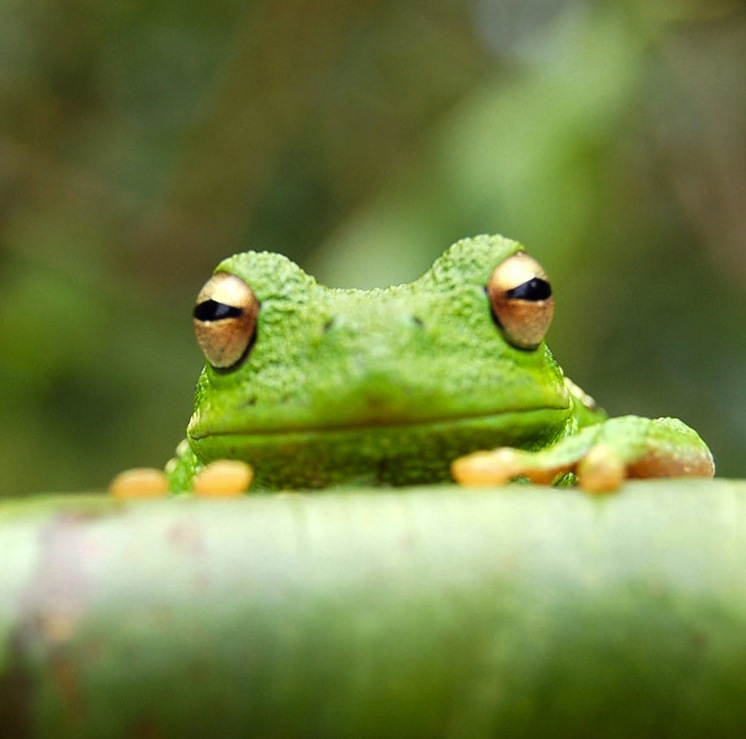
\includegraphics[width=0.45\textwidth]{figures/frog.jpg}
\caption{\label{fig:categorical}Categorical Data.}
\end{figure}

bla

%%%%%%%%%%%%%%%%%%%%%%%%%%%%%%%%%%%%%%%%%%%%%%%%%%%%%%%%%%%%%%%%%%%%%%%%%%%%%%%%%%%%%%%%
%% DATA PREPROCESSING
%%%%%%%%%%%%%%%%%%%%%%%%%%%%%%%%%%%%%%%%%%%%%%%%%%%%%%%%%%%%%%%%%%%%%%%%%%%%%%%%%%%%%%%%

\section{Data Preprocessing}
\label{sec:data_preprocessing}
In this section, I will preprocess the data to create a better representation of customers by performing a scaling on the data and detecting (and optionally removing) outliers. Preprocessing data is often times a critical step in assuring that results I obtain from my analysis are significant and meaningful.

%%%%%%%%%%%%%%%%%%%%%%%%%%%%%%%%%%%%%%%%%%%%%%%%%%%%%%%%%%%%%%%%%%%%%%%%%%%%%%%%%%%%%%%%
%% FEATURE TRANSFORMATION
%%%%%%%%%%%%%%%%%%%%%%%%%%%%%%%%%%%%%%%%%%%%%%%%%%%%%%%%%%%%%%%%%%%%%%%%%%%%%%%%%%%%%%%%

\section{Feature Transformation}
\label{sec:feature_transformation}
In this section I will use principal component analysis (PCA) to draw conclusions about the underlying structure of the wholesale customer data. Since using PCA on a dataset calculates the dimensions which best maximize variance, we will find which compound combinations of features best describe customers.


%%%%%%%%%%%%%%%%%%%%%%%%%%%%%%%%%%%%%%%%%%%%%%%%%%%%%%%%%%%%%%%%%%%%%%%%%%%%%%%%%%%%%%%%
%% CLUSTERING
%%%%%%%%%%%%%%%%%%%%%%%%%%%%%%%%%%%%%%%%%%%%%%%%%%%%%%%%%%%%%%%%%%%%%%%%%%%%%%%%%%%%%%%%

\section{Clustering}
\label{sec:clustering}
In this section, I will choose to use either a K-Means clustering algorithm or a Gaussian Mixture Model clustering algorithm to identify the various customer segments hidden in the data. I will then recover specific data points from the clusters to understand their significance by transforming them back into their original dimension and scale.


%%%%%%%%%%%%%%%%%%%%%%%%%%%%%%%%%%%%%%%%%%%%%%%%%%%%%%%%%%%%%%%%%%%%%%%%%%%%%%%%%%%%%%%%
%% CONCLUSION
%%%%%%%%%%%%%%%%%%%%%%%%%%%%%%%%%%%%%%%%%%%%%%%%%%%%%%%%%%%%%%%%%%%%%%%%%%%%%%%%%%%%%%%%

\section{Conclusion}
\label{sec:conclusion}


%%%%%%%%%%%%%%%%%%%%%%%%%%%%%%%%%%%%%%%%%%%%%%%%%%%%%%%%%%%%%%%%%%%%%%%%%%%%%%%%%%%%%%%%
%% REFLECTION
%%%%%%%%%%%%%%%%%%%%%%%%%%%%%%%%%%%%%%%%%%%%%%%%%%%%%%%%%%%%%%%%%%%%%%%%%%%%%%%%%%%%%%%%

\section{Reflection}
\label{sec:reflection}
Bla bla bla




\bibliographystyle{plain}
% or try abbrvnat or unsrtnat
\bibliography{bibliography/biblio.bib}
\end{document}
